% SPDX-License-Identifier: Apache-2.0 OR MIND-UCAL-1.0
% © James Ross Ω FLYING•ROBOTS <https://github.com/flyingrobots>
\documentclass{aion}

% ------------------------------------------------------------
% Metadata for this paper
% ------------------------------------------------------------
\renewcommand{\papertitle}{WARP Graphs---WARP Core: Deterministic Graph Rewrite Simulation Engine}
\renewcommand{\papernumber}{Paper VII}
\renewcommand{\paperdate}{Januray 2026}

\renewcommand{\paperauthor}{James Ross}
\renewcommand{\paperaffiliation}{Independent Researcher}
\renewcommand{\paperorcid}{0009-0006-0025-7801}
\renewcommand{\paperdoi}{10.5281/zenodo.18038297}

% ------------------------------------------------------------
% Packages (local to this paper)
% ------------------------------------------------------------
\usepackage{float}
\usepackage{mathtools}
\usepackage{tabularx}
\usepackage{tikz}
\usepackage{tikz-cd}
\usetikzlibrary{arrows.meta,positioning,decorations.pathreplacing,fit,calc}

% SPDX-License-Identifier: Apache-2.0 OR MIND-UCAL-1.0
% © James Ross Ω FLYING•ROBOTS <https://github.com/flyingrobots>
% Macros for the WARPs paper
% Shared commands to keep notation consistent across the manuscript.
\RequirePackage{url}
\DeclareRobustCommand{\AION}{\textrm{AI}\ensuremath{\Omega}\textrm{N}}
\DeclareRobustCommand{\AIONProjectURL}{\url{https://github.com/flyingrobots/aion}}

% WARP term: small caps in prose, italic in math.
% Force upright small caps in text to avoid missing scit font shapes.
\DeclareRobustCommand{\WARP}{\ifmmode\mathit{WARP}\else{\upshape\scshape warp}\fi}


% ------------------------------------------------------------
% Notation shortcuts (guarded to avoid clashes with other papers)
% ------------------------------------------------------------
\ifdefined\WCat\else\newcommand{\WCat}{\mathcal{W}}\fi
\ifdefined\Hist\else\DeclareMathOperator{\Hist}{Hist}\fi
\ifdefined\Trans\else\DeclareMathOperator{\Trans}{Trans}\fi
\ifdefined\DL\else\DeclareMathOperator{\DL}{DL}\fi
\ifdefined\Dist\else\DeclareMathOperator{\Dist}{Dist}\fi
\ifdefined\To\else\newcommand{\To}{\to}\fi

\newcommand{\WState}{\mathsf{WState}}
\newcommand{\Tr}{\mathsf{Tr}}
\newcommand{\Labels}{\mathsf{Labels}}
\newcommand{\Apply}{\mathsf{Apply}}

\DeclareMathOperator{\MW}{MW}
\DeclareMathOperator{\Path}{Path}
\DeclareMathOperator{\Obj}{Obj}
\DeclareMathOperator{\Mor}{Mor}
\DeclareMathOperator{\dom}{dom}
\DeclareMathOperator{\cod}{cod}

\newcommand{\Ruliad}{\mathcal{R}}
\newcommand{\Chronos}{\mathsf{Chronos}}
\newcommand{\Kairos}{\mathsf{Kairos}}
\newcommand{\Aion}{\mathsf{Aion}}

% \newcommand{\AION}{\mathdf{AI\upOmegaN}}

% Paper I used \sectionbreak; provide a default in case the class doesn't.
\providecommand{\sectionbreak}{\clearpage}

% Avoid duplicate hyperlink anchors for figures
\makeatletter
\renewcommand{\theHfigure}{\thesection.\arabic{figure}}
\makeatother

\usetikzlibrary{backgrounds}

\begin{document}

\AIONFrontMatter{This paper outlines the architecture of the \textit`'{WARP Core} deterministic graph rewrite engine, a high-performance, real-time simulation engine with bit-level perfect deterministism, embarassingly-high coucurrency, and first-class time travel, by construction.
}

% ============================================================
\section{Introduction}
\label{sec:intro}

To conclude the \textbf{\AION{} Foundations Series}, we describe the construction of the WARP Core, a real-time deterministic graph rewrite simulation engine. This technology is already running this project's homepage, https://flyingrobots.dev, known herein as the "WARPSite"---a "website" powered by the WARP
Paper~I introduces \WARP\ graphs as a minimal recursively nested state object~\cite{Ros25a}.
Paper~II defines a deterministic multiway semantics (via a two-plane DPO discipline) so that
executions become replayable \emph{worldlines}~\cite{Ros25b}.
Paper~III shows that deterministic worldlines admit a boundary representation:
a \emph{provenance payload} is sufficient to reconstruct the full interior derivation volume
(\emph{computational holography})~\cite{Ros25c}.

This paper addresses the remaining mathematical question: \emph{how should a computation be compared across observers?}
In practice, consumers rarely require a raw microstep-by-microstep derivation. Engineering use-cases demand derived views:
summaries for interpretation, invariants for compilation, provenance for audit, and counterfactual branches for adversarial analysis.
These viewpoints correspond to different \emph{observers} of the same underlying history.

The correct comparison problem is not ``which observer is right?'' but:
\begin{quote}
\emph{Given two observers that emit different trace languages, what is the cost of translating between them
under explicit resource constraints, and how much distortion is unavoidable?}
\end{quote}
We operationalise this as a geometry on observer space: a distance defined by translator description length
(MDL) plus trace distortion. This distance is \emph{budgeted}: two observers may be equivalent under unbounded
resources but far apart at finite time/memory budgets.

\paragraph{Context within the Series.}
Paper~V is about ethics: what perfect provenance implies for accountability, privacy, and power.
Paper~VI is about architecture: how to implement the semantics as a system.
Paper~IV is therefore the final mathematics-oriented paper in the series.
Accordingly, we take the opportunity to give the Ruliad connection and observer geometry the full formal weight
they require, rather than deferring mathematical structure to later papers.

\paragraph{Contributions.}
The contributions of this paper are:

\begin{enumerate}[leftmargin=*]
  \item A stand-alone account of \emph{history categories} for \WARP\ rewriting, relating deterministic worldlines
        to multiway systems (\S\ref{sec:prelim}, \S\ref{sec:multiway}).
  \item A formal definition of \emph{observers} as resource-bounded functors out of $\Hist(\mathcal{U},R)$ into an
        observation space, including boundary-versus-bulk observer pairs induced by holography (\S\ref{sec:observers}).
  \item A translation framework between observers, equipped with MDL description length~\cite{Ris78} and
        trace distortion, together with explicit assumptions needed for compositionality (\S\ref{sec:translators}).
  \item The definition of the \emph{rulial distance} $D_{\tau,m}$ and its core properties:
        non-negativity, symmetry, monotonicity under budget relaxation, and a triangle inequality up to a constant
        overhead inherited from prefix coding, together with a Lawvere-metric/enriched-category interpretation of directed cost
        (\S\ref{sec:rulial}).
  \item A formalisation of the Chronos--Kairos--Aion triad as a three-layer time model embedded in the multiway space,
        and an interpretation of rulial distance as ``frame separation'' in the Ruliad (\S\ref{sec:multiway}).
  \item A minimal temporal logic aligned with Chronos--Kairos--Aion, with concrete liveness/reconciliation examples and a
        transport lemma relating temporal satisfaction to observer translation cost (\S\ref{sec:multiway}).
\end{enumerate}

\paragraph{Scope management.}
We deliberately do \emph{not} attempt to axiomatise a single canonical trace metric,
nor do we claim that MDL gives an optimal notion of semantic similarity for all domains.
Our aim is narrower and foundational: to provide a mathematically explicit, computable mechanism that turns
\emph{translation cost} into geometry, so that later work can specialise it to concrete trace languages and security goals.

\paragraph{Roadmap.}
We begin by restating the minimal background from Papers~I--III needed for a stand-alone reading (\S\ref{sec:prelim}).
We then formalise observers as resource-bounded functors out of history categories and motivate canonical observer families
induced by holography (\S\ref{sec:observers}).
Next we introduce translators, MDL description length, and lifted distortion as the ingredients for a quantitative comparison
of observers (\S\ref{sec:translators}).
Rulial distance is defined and analysed in \S\ref{sec:rulial}, including the Lawvere-metric/enriched-category interpretation of
directed cost (\S\ref{subsec:lawvere}).
We then connect deterministic worldlines to multiway systems and the Ruliad, formalise the Chronos--Kairos--Aion time model,
and develop a minimal temporal logic whose semantics range over worldlines and branching histories (\S\ref{sec:multiway},
\S\ref{subsec:temporal-logic}).
Finally, we summarise related work (\S\ref{sec:related}), discuss implications and open directions (\S\ref{sec:outlook}),
and provide a notation summary (\S\ref{sec:notation}).

\sectionbreak

% ============================================================
\section{Preliminaries and Standing Assumptions}
\label{sec:prelim}

We briefly restate the fragments of Papers~I--III needed for a self-contained treatment.
Throughout, we adopt the deterministic replay discipline of Paper~II (fixed boundary data determines a unique committed tick worldline)
and the boundary encoding of Paper~III.

\subsection[Warp states and deterministic worldlines]{\textnormal{\textsc{Warp}} states and deterministic worldlines}
\label{subsec:prelim-warps}

A \WARP\ graph is a finite directed multigraph whose vertices and edges carry recursively attached \WARP\ graphs~\cite{Ros25a}.
A \emph{\WARP\ state} $U\in\WState$ is a typed open graph skeleton together with recursively attached \WARP\ states on each vertex and edge.
We write $\skel(U)$ for the skeleton component.

Deterministic evolution is expressed in ticks.
Let $\Labels$ denote the space of tick patches: finite records sufficient to advance the state by one tick under the deterministic semantics of Paper~II.
Write
\[
  \Apply : \WState \times \Labels \rightharpoonup \WState
\]
	for the deterministic tick-application function.
	A \emph{tick patch} is an element $\mu\in\Labels$ (intended to be applied via $\Apply$).
	Intuitively, a tick patch is the serialised record of the within-tick batch committed at that tick.
	A \emph{tick} is the unit of concurrent evolution: it groups attachment-plane rewrites together with a scheduler-selected batch of independent skeleton rewrites, committed atomically (Paper~II, Def.~4.2).
	A deterministic worldline is a sequence
\[
  U_0 \;\Rightarrow\; U_1 \;\Rightarrow\; \cdots \;\Rightarrow\; U_n
\qquad\text{with}\qquad
U_{i+1}=\Apply(U_i,\mu_i)
\]
whenever defined~\cite{Ros25b}.
Paper~II shows how to construct such an $\Apply$ from DPO rewriting in adhesive categories under a two-plane discipline,
and how to package scheduling decisions so that replay is bit-level deterministic.

\subsection{Boundary encoding and wormholes}
\label{subsec:prelim-holography}

Paper~III introduces a \emph{provenance payload}
\[
  P=(\mu_0,\ldots,\mu_{n-1})
\]
and the boundary encoding $(U_0,P)$~\cite{Ros25c}.
Under patch sufficiency,\footnote{Patch sufficiency is the condition that $(U_0,P)$ uniquely determines the interior worldline under the deterministic semantics.}
$(U_0,P)$ reconstructs the interior worldline uniquely.
A \emph{wormhole} is a provenance-preserving compression of a multi-tick segment into a single edge labelled by a sub-payload.
For the present paper, holography induces two natural classes of observers:
\begin{itemize}[leftmargin=*]
  \item \emph{bulk observers} that inspect some or all of the interior worldline; and
  \item \emph{boundary observers} that operate only on the compact boundary artefact $(U_0,P)$.
\end{itemize}
Rulial distance will quantify the cost of translating between these viewpoints.

\subsection{Multiway graphs and history categories}
\label{subsec:prelim-history}

Fix a universe $\mathcal{U}\subseteq\WState$ and a rule pack $R$ (a finite set of rewrite rules plus the fixed typing/open-graph discipline).
The associated \emph{multiway graph} is the directed graph
\[
  \MW(\mathcal{U},R) = (V,E)
\]
whose vertices are states $V=\mathcal{U}$ and whose directed edges are individual rewrite steps generated by $R$
(including alternative matches and orderings where applicable).
In general $\MW(\mathcal{U},R)$ branches and merges.

\begin{definition}[History category]\label{def:hist-category}
Let $\MW(\mathcal{U},R)$ be a multiway graph.
Its \emph{history category} $\Hist(\mathcal{U},R)$ is the path category of $\MW(\mathcal{U},R)$:
\begin{itemize}[leftmargin=*]
  \item objects are states $U\in\mathcal{U}$;
  \item morphisms $h:U\to V$ are finite directed paths in $\MW(\mathcal{U},R)$ from $U$ to $V$;
  \item composition is path concatenation.
\end{itemize}
\end{definition}

\begin{remark}[Deterministic worldlines as functors]
A deterministic worldline $U_0\Rightarrow U_1\Rightarrow\cdots$ defines a functor
$W:\mathbb{N}\to\Hist(\mathcal{U},R)$ sending $i\mapsto U_i$ and $(i\to i{+}1)\mapsto (U_i\to U_{i+1})$.
The determinism discipline of Paper~II can be understood as selecting a unique such functor for fixed boundary data.
We later formalise its finite restriction as the Chronos functor (Definition~\ref{def:chronos} in \S\ref{subsec:chronos-kairos-aion}).
\end{remark}

\sectionbreak

% ============================================================
\section{Observers}
\label{sec:observers}

Observers are the interface between a \WARP\ history and a consumer.
We treat observers as functors out of the history category into a structured space of traces.

\subsection{Observation spaces}
\label{subsec:obs-spaces}

An \emph{observation space} is an object that supports:
(i) a notion of trace value; and (ii) a distortion measure between traces.
The minimal structure we require is a set $\Tr$ equipped with a metric (or pseudometric)
\[
  \mathrm{dist}_{\mathrm{tr}} : \Tr\times\Tr\to\mathbb{R}_{\ge 0}.
\]
In applications, $\Tr$ may be:
symbol streams, labelled paths, graphs of causal dependencies, certificates, or slices of provenance payloads.

When it is convenient to keep categorical structure explicit, we may regard $\Tr$ as the object set of a category $\mathcal{Y}$
and work objectwise. Nothing in the core definitions requires nontrivial morphisms in $\mathcal{Y}$; the geometry is carried
by $\mathrm{dist}_{\mathrm{tr}}$.

\subsection{Observers as budgeted functors}
\label{subsec:obs-functors}

\begin{definition}[Observer]\label{def:observer}
Fix $\Hist(\mathcal{U},R)$ and an observation space $(\Tr,\mathrm{dist}_{\mathrm{tr}})$.
An \emph{observer} is a functor
\[
  O : \Hist(\mathcal{U},R)\to \Tr,
\]
where we regard $\Tr$ as a discrete category.
Operationally, $O$ is realised by an algorithm that maps any derivation path $h$ to a trace value $O(h)$.
\end{definition}

\begin{definition}[Resource-bounded observer]\label{def:budgeted-observer}
Let $(\tau,m)$ be time and memory budgets (in any fixed machine model).
An observer $O$ is \emph{$(\tau,m)$-bounded} if it admits an implementation that, on any history input $h$ in its domain,
runs within time $\tau$ and memory $m$.
\end{definition}

\begin{remark}[Why we bound observers]
Without explicit budgets, all observers collapse into an uninformative equivalence: ``compute the full worldline and output it''.
Budgets ensure the geometry respects real computational constraints: replaying a wormhole is algorithmically simple
(low description length) but may be infeasible at small $\tau$.
\end{remark}

\subsection{Canonical observer families induced by holography}
\label{subsec:obs-holography}

Holographic boundary encoding induces a practical taxonomy of observers:
\begin{itemize}[leftmargin=*]
  \item \emph{boundary observers} that inspect only $(U_0,P)$ (or its authenticated packaging such as a BTR);
  \item \emph{bulk observers} that inspect interior states, matches, receipts, or causal cones; and
  \item \emph{semantic observers} that collapse syntactic evolution into invariant properties (types, safety checks, query semantics).
\end{itemize}

\begin{example}[Boundary vs bulk]\label{ex:boundary-bulk}
Let $O_{\partial}$ map a history $h$ to the boundary artefact $(U_0,P)$ that generates it,
and let $O_{\mathrm{bulk}}$ map $h$ to the full state sequence $(U_0,\ldots,U_n)$.
There is a natural translator $T_{\mathrm{replay}}$ from $O_{\partial}$ to $O_{\mathrm{bulk}}$ given by deterministic replay.
Its \emph{description length} is small (it is essentially the interpreter $\Apply$),
but its \emph{time cost} grows with the length of $P$.
This example will be revisited in \S\ref{subsec:rulial-budget-effects}.
\end{example}

\subsection{Observer projections of wormholes}
\label{subsec:obs-projections}

Given a wormhole boundary encoding $(U_0,P)$, different observers may:
\begin{itemize}[leftmargin=*]
  \item expose only coarse-grained stages of $P$ (e.g.\ AST$\to$IR$\to$plan);
  \item restrict to semantic effects (e.g.\ schema and invariants);
  \item highlight only adversarial or counterfactual branches;
  \item or inspect every microstep.
\end{itemize}

\begin{figure}[t]
  \centering
  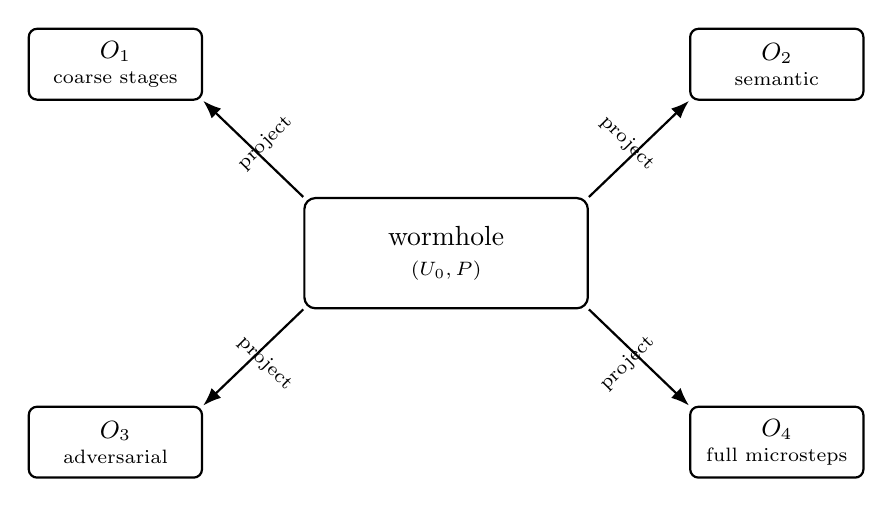
\begin{tikzpicture}[
      wormhole/.style={rectangle,draw=black,thick,rounded corners,
                       minimum width=36mm,minimum height=14mm,align=center},
      observer/.style={rectangle,draw=black,thick,rounded corners=3pt,
                       minimum width=22mm,minimum height=9mm,align=center,font=\small},
      arrow/.style={-Latex,thick,draw=black},
      >=Latex
    ]

    % Central wormhole
    \node[wormhole] (W) at (0,0)
      {wormhole\\[-1pt]
       \scriptsize $(U_0,P)$};

    % Observers
    \node[observer] (O1) at (-4.2,2.4) {$O_1$\\[-2pt]\scriptsize coarse stages};
    \node[observer] (O2) at (4.2,2.4) {$O_2$\\[-2pt]\scriptsize semantic};
    \node[observer] (O3) at (-4.2,-2.4) {$O_3$\\[-2pt]\scriptsize adversarial};
    \node[observer] (O4) at (4.2,-2.4) {$O_4$\\[-2pt]\scriptsize full microsteps};

    % Projections
    \draw[arrow] (W.north west) -- (O1.south east);
    \draw[arrow] (W.north east) -- (O2.south west);
    \draw[arrow] (W.south west) -- (O3.north east);
    \draw[arrow] (W.south east) -- (O4.north west);

    % Labels on arrows
    \node[rotate=45,font=\scriptsize] at (-2.3,1.4) {project};
    \node[rotate=-45,font=\scriptsize] at (2.3,1.4) {project};
    \node[rotate=-45,font=\scriptsize] at (-2.3,-1.4) {project};
    \node[rotate=45,font=\scriptsize] at (2.3,-1.4) {project};

  \end{tikzpicture}
  \caption{Multiple observers projecting the same wormhole boundary $(U_0,P)$ into different trace formats.
  The rulial distance measures the complexity of translating between such views, balancing translator description length
  against residual distortion.}
  \label{fig:observer-projections}
\end{figure}

\sectionbreak

% ============================================================
\section{Translators, MDL Complexity, and Distortion}
\label{sec:translators}

To compare observers we require a compositional notion of translation, a complexity measure for translators,
and a distortion measure between outputs.

\subsection{Translators}
\label{subsec:translators-def}

Let $O_1,O_2:\Hist(\mathcal{U},R)\to\Tr$ be observers into a common trace space.
A translator should map traces produced by $O_1$ into traces in the format of $O_2$.

\begin{definition}[Translator]\label{def:translator}
A \emph{translator} from $O_1$ to $O_2$ is an algorithmic operator
\[
  T_{12} : \Tr \to \Tr
\]
such that $T_{12}\circ O_1$ is a well-defined observer and is intended to approximate $O_2$.
We write $T_{12}\in\Trans(O_1,O_2)$.
\end{definition}

\begin{remark}[Why we translate by post-composition]
This definition makes typing explicit: $T_{12}\circ O_1$ is an observer with the same domain as $O_2$.
If one prefers to keep the functor category $\Tr^{\Hist(\mathcal{U},R)}$ explicit, a translator can be regarded as an endofunctor
on $\Tr$ together with the induced action on observers by post-composition.
\end{remark}

\begin{definition}[Budgeted translators]\label{def:budgeted-trans}
For budgets $(\tau,m)$, let $\Trans_{\tau,m}(O_1,O_2)\subseteq\Trans(O_1,O_2)$ denote the translators
realisable within those budgets.
\end{definition}

\begin{assumption}[Budgeted translator axioms]\label{ass:budgeted-trans}
For each budget pair $(\tau,m)$:
\begin{enumerate}[leftmargin=*]
  \item \emph{Identity.} For every observer $O$, the identity translator $I$ belongs to $\Trans_{\tau,m}(O,O)$, and we normalise
        codes so that $\DL(I)=0$.
  \item \emph{Composition.} If $T_{12}\in\Trans_{\tau,m}(O_1,O_2)$ and $T_{23}\in\Trans_{\tau,m}(O_2,O_3)$, then
        \[
          T_{23}\circ T_{12}\in\Trans_{\tau,m}(O_1,O_3).
        \]
\end{enumerate}
\end{assumption}

\begin{example}[SQL $\leftrightarrow$ AST]\label{ex:sql-ast}
Consider a \WARP\ universe modelling a database query planner.
Observer $O_1$ outputs a trace of AST transformations, while observer $O_2$ outputs only the initial SQL string
and a final execution summary.
A translator $T_{12}$ must compile an AST evolution into a SQL-like summary, while $T_{21}$ must infer a plausible AST evolution
consistent with SQL and execution effects.
The description lengths $\DL(T_{12}),\DL(T_{21})$ and their residual distortions quantify the separation of these two views.
\end{example}

\subsection{MDL and description length}
\label{subsec:mdl}

We measure translator complexity using MDL: a translator is ``simple'' if it admits a short prefix-free description.

\begin{definition}[Description length]\label{def:dl}
Fix a prefix-free code over translator programmes.
For a translator $T$, let $\DL(T)\in\mathbb{R}_{\ge 0}$ denote the length of its code word.
\end{definition}

The constant-overhead behaviour of prefix codes gives the subadditivity we require.

\begin{assumption}[Subadditivity up to a constant]\label{ass:dl-subadd}
There exists a constant $c\ge 0$ such that for any composable translators $T_{12},T_{23}$ we have
\[
  \DL(T_{23}\circ T_{12}) \le \DL(T_{12}) + \DL(T_{23}) + c.
\]
\end{assumption}

\begin{remark}[On the constant $c$]
The constant $c$ is the code overhead required to describe ``run $T_{12}$ then $T_{23}$'' under the chosen universal coding scheme.
MDL theory~\cite{Ris78} (and related invariance results for prefix complexity~\cite{LiVitanyi2019}) justify treating such overhead as $O(1)$:
it does not scale with the size of the translators being composed.
\end{remark}
\begin{remark}[Relation to information distance and rate--distortion]
At $\lambda\to\infty$ with the constraint $\Dist(O_2,T\circ O_1)=0$, the directed cost
reduces to the description length of the shortest exact translator from $O_1$ to $O_2$.
The resulting symmetrised distance is closely related in spirit to \emph{algorithmic information distance}:
the Kolmogorov-style cost of converting one description into another~\cite{Bennett98,LiVitanyi2019}.
At finite $\lambda$, the objective is an MDL-flavoured instance of a rate--distortion trade-off:
we pay \emph{rate} (translator description length) to purchase lower residual distortion.
\end{remark}


\subsection{Trace distortion and lifted observer distortion}
\label{subsec:distortion}

Fix a metric (or pseudometric) $\mathrm{dist}_{\mathrm{tr}}$ on trace space $\Tr$.
We lift it to a distortion between observers by taking a supremum over histories.

\begin{definition}[Lifted distortion]\label{def:dist-lift}
For observers $O,O':\Hist(\mathcal{U},R)\to\Tr$, define
\[
  \Dist(O,O') \;:=\; \sup_{h\in\Mor(\Hist(\mathcal{U},R))}\,
  \mathrm{dist}_{\mathrm{tr}}\bigl(O(h),O'(h)\bigr).
\]
\end{definition}

\begin{assumption}[Bounded diameter]\label{ass:bounded-diameter}
All observers under comparison take values in a common trace space $\Tr$ of uniformly bounded diameter,
so that $\Dist(O,O')$ is finite.
\end{assumption}

\begin{assumption}[Non-expansive translators]\label{ass:lipschitz}
Post-composition by any translator is $1$-Lipschitz:
\[
  \Dist(T\circ O,\, T\circ O') \le \Dist(O,O')
\]
for all translators $T$ and observers $O,O'$.
\end{assumption}

\begin{remark}[Alternative liftings]
The supremum lifting is conservative: it protects against worst-case histories and adversarial inputs.
In statistical settings we may instead use an expected distortion over a distribution on histories, or restrict to histories within a time cone.
Our results adapt to any lifting that preserves the triangle inequality and non-expansiveness properties used in \S\ref{sec:rulial}.
\end{remark}

\sectionbreak

% ============================================================
\section{Rulial Distance}
\label{sec:rulial}

We now define the rulial distance and prove its core properties.
Throughout we fix a weighting parameter $\lambda>0$ trading off translator complexity against residual distortion.

\subsection{Directed and symmetrised distance}

It is useful to separate the directed translation problem from its symmetrisation.

\begin{definition}[Directed rulial cost]\label{def:directed}
For observers $O_1,O_2$ define the directed cost
\[
  \vec{D}_{\tau,m}(O_1\!\to\! O_2)
  :=
  \inf_{T_{12}\in\Trans_{\tau,m}(O_1,O_2)}
  \Bigl(\DL(T_{12}) + \lambda\,\Dist(O_2,\,T_{12}\circ O_1)\Bigr),
\]
with the convention that the infimum over an empty set is $+\infty$.
\end{definition}

\begin{definition}[Rulial distance]\label{def:rulial}
The (symmetrised) \emph{rulial distance} is
\[
  D_{\tau,m}(O_1,O_2)
  :=
  \vec{D}_{\tau,m}(O_1\!\to\! O_2)
  \;+\;
  \vec{D}_{\tau,m}(O_2\!\to\! O_1).
\]
Equivalently, expanding the two infima yields the joint infimum formulation used in earlier drafts:
\[
  D_{\tau,m}(O_1,O_2)
   = \inf_{\substack{
         T_{12}\in\Trans_{\tau,m}(O_1,O_2)\\
         T_{21}\in\Trans_{\tau,m}(O_2,O_1)}}
      \Bigl(
        \DL(T_{12}) + \DL(T_{21})
        + \lambda \bigl(
           \Dist(O_2, T_{12}\circ O_1) +
           \Dist(O_1, T_{21}\circ O_2)
        \bigr)
      \Bigr).
\]
\end{definition}

\subsection{Basic properties}

\begin{theorem}[Basic properties]\label{thm:rulial-basic}
For all observers $O_1,O_2$ and budgets $(\tau,m)$:
\begin{enumerate}[leftmargin=*]
  \item $D_{\tau,m}(O_1,O_2)\ge 0$;
  \item $D_{\tau,m}(O_1,O_2)=D_{\tau,m}(O_2,O_1)$;
  \item $D_{\tau,m}(O,O)=0$ for every observer $O$.
\end{enumerate}
\end{theorem}

\begin{proof}
Non-negativity follows because $\DL\ge 0$ and $\Dist\ge 0$.
Symmetry holds by definition of $D_{\tau,m}$ as the sum of two directed terms.
For reflexivity, the identity translator $I$ is admissible by Assumption~\ref{ass:budgeted-trans} and
satisfies $\DL(I)=0$ and $\Dist(O,I\circ O)=0$, so both directed costs vanish.
\end{proof}

\begin{corollary}[Observer equivalence]\label{cor:observer-equivalence}
Let $O_1,O_2$ be observers.
Then $D_{\tau,m}(O_1,O_2)=0$ if and only if there exist translators
$T_{12}\in\Trans_{\tau,m}(O_1,O_2)$ and $T_{21}\in\Trans_{\tau,m}(O_2,O_1)$ such that:
\begin{enumerate}[leftmargin=*]
  \item $\Dist(O_2, T_{12}\circ O_1)=0$ and $\Dist(O_1, T_{21}\circ O_2)=0$; and
  \item $\DL(T_{12})$ and $\DL(T_{21})$ are bounded by a constant independent of the histories under consideration.
\end{enumerate}
In this case the observers are equivalent under the rulial geometry: they differ only by constant-overhead,
distortion-free translation.
\end{corollary}

\begin{proof}[Proof sketch]
If such translators exist then both directed costs are bounded by constants independent of the histories (distortion is $0$ and description length is constant),
so $D_{\tau,m}(O_1,O_2)$ is bounded by a constant.
Under the constant-overhead convention of the remark below, we identify such constant separation with $0$, yielding $D_{\tau,m}(O_1,O_2)=0$.
Conversely, if $D_{\tau,m}(O_1,O_2)=0$ then (by definition of $D_{\tau,m}$ as the sum of two directed costs)
both directed costs vanish modulo constant overhead, hence there exist translators in both directions with
zero residual distortion and constant description length, as claimed.
\end{proof}

\begin{remark}
Observer equivalence is defined modulo constant description overhead; exact zero-length translators are not required and depend on the choice of coding scheme.
\end{remark}

\subsection{Monotonicity under budget relaxation}
\label{subsec:rulial-monotone}

The budgeted nature of rulial distance is essential: it distinguishes translations that are short in description length
but exceed available time/memory resources from those that are admissible under the deployment constraints.

\begin{proposition}[Budget monotonicity]\label{prop:budget-monotone}
If $(\tau',m')\succeq(\tau,m)$ (i.e.\ $\tau'\ge\tau$ and $m'\ge m$) then
\[
  D_{\tau',m'}(O_1,O_2) \le D_{\tau,m}(O_1,O_2).
\]
\end{proposition}

\begin{proof}
By definition, $\Trans_{\tau,m}(O_i,O_j)\subseteq \Trans_{\tau',m'}(O_i,O_j)$ under budget relaxation,
so the infimum is taken over a larger set and cannot increase.
\end{proof}

\subsection{Triangle inequality up to a constant}
\label{subsec:rulial-triangle}

\begin{theorem}[Triangle inequality up to additive slack]\label{thm:rulial-triangle}
Assume:
\begin{enumerate}[leftmargin=*]
  \item Assumption~\ref{ass:dl-subadd} (subadditivity of $\DL$ up to constant $c$);
  \item $\Dist$ is a metric on observers (triangle inequality) and translators are non-expansive
        (Assumption~\ref{ass:lipschitz});
  \item budget classes are closed under composition (Assumption~\ref{ass:budgeted-trans}).
\end{enumerate}
Then for all observers $O_1,O_2,O_3$ we have
\[
  D_{\tau,m}(O_1,O_3) \le D_{\tau,m}(O_1,O_2) + D_{\tau,m}(O_2,O_3) + 2c.
\]
\end{theorem}

\begin{proof}
Fix $\varepsilon>0$ and choose near-optimal translators for the two distances:
pick $T_{12},T_{21}$ such that the objective for $D_{\tau,m}(O_1,O_2)$ is within $\varepsilon/2$ of the infimum,
and $T_{23},T_{32}$ similarly for $D_{\tau,m}(O_2,O_3)$.
By closure under composition, $T_{13}=T_{23}\circ T_{12}$ and $T_{31}=T_{21}\circ T_{32}$
are admissible budgeted translators.

Subadditivity gives $\DL(T_{13})\le\DL(T_{12})+\DL(T_{23})+c$ and
$\DL(T_{31})\le\DL(T_{21})+\DL(T_{32})+c$.
For distortion, the triangle inequality and non-expansiveness yield
\begin{align*}
  \Dist(O_3,\,T_{13}\circ O_1)
    &= \Dist(O_3,\,T_{23}\circ T_{12}\circ O_1)\\
    &\le \Dist(O_3,\,T_{23}\circ O_2) + \Dist(T_{23}\circ O_2,\,T_{23}\circ T_{12}\circ O_1)\\
    &\le \Dist(O_3,\,T_{23}\circ O_2) + \Dist(O_2,\,T_{12}\circ O_1),
\end{align*}
and similarly for $\Dist(O_1,\,T_{31}\circ O_3)$.
Summing the bounds and using near-optimality yields the stated inequality up to $\varepsilon$.
Letting $\varepsilon\to 0$ completes the proof.
\end{proof}

\begin{remark}[Quasi-pseudometric]
Together with Theorem~\ref{thm:rulial-basic}, Theorem~\ref{thm:rulial-triangle} makes $D_{\tau,m}$ a
quasi-pseudometric: it satisfies all pseudometric axioms except that the triangle inequality holds only up to an additive constant $2c$.
In practice $c$ is a small, fixed prefix-coding overhead; it may also be absorbed into $\lambda$ if desired.
The geometry is most informative when translation costs scale nontrivially with history size, or when comparing asymptotically distinct observer classes (e.g.\ $O(1)$ vs $O(N)$), in which regime the constant $c$ becomes negligible.
\end{remark}

\subsection{Lawvere-metric (enriched category) viewpoint}
\label{subsec:lawvere}

The symmetrised distance $D_{\tau,m}$ is convenient for neighbourhoods and ``frame separation'',
but the underlying translation problem is inherently \emph{directed}:
decompressing a boundary view into a bulk view can be infeasible under strict budgets,
whereas projection from bulk into boundary is typically admissible under the same budgets.
This asymmetry is captured by Lawvere's observation that metric spaces are categories enriched in
the monoidal poset $([0,\infty],\ge,+,0)$~\cite{Lawvere73,Kelly82}.

\begin{definition}[Lawvere metric space]\label{def:lawvere-metric}
A \emph{Lawvere metric space} is a category enriched over the monoidal poset $([0,\infty],\ge,+,0)$.
Concretely, it is a collection of objects together with a function $d(x,y)\in[0,\infty]$ such that:
(i) $d(x,x)=0$ for all $x$; and (ii) $d(x,z)\le d(x,y)+d(y,z)$ for all $x,y,z$.
No symmetry condition is imposed; $d(x,y)$ and $d(y,x)$ may differ.
The value $+\infty$ is permitted and represents ``no morphism'' (infeasible translation).
\end{definition}

\begin{definition}[Directed rulial hom]\label{def:lawvere-hom}
Fix budgets $(\tau,m)$.
For observers $O_1,O_2$ define the \emph{directed hom-value}
\[
  d_{\tau,m}(O_1,O_2) \;:=\; \vec{D}_{\tau,m}(O_1\!\to\!O_2)\in[0,\infty],
\]
with the convention $d_{\tau,m}(O_1,O_2)=+\infty$ when $\Trans_{\tau,m}(O_1,O_2)=\varnothing$.
The symmetrised rulial distance is the induced symmetrisation
$D_{\tau,m}(O_1,O_2)=d_{\tau,m}(O_1,O_2)+d_{\tau,m}(O_2,O_1)$.
\end{definition}

For notational convenience, we treat $\vec{D}_{\tau,m}(O_1\!\to\!O_2)$ and $d_{\tau,m}(O_1,O_2)$ as interchangeable;
we use $d_{\tau,m}$ when emphasising the Lawvere-enriched interpretation.

\begin{proposition}[Composition as triangle inequality]\label{prop:lawvere-triangle}
Assume:
(i) Assumption~\ref{ass:dl-subadd};
(ii) $\Dist$ satisfies the triangle inequality and translators are non-expansive (Assumption~\ref{ass:lipschitz});
and (iii) budget classes are closed under composition (Assumption~\ref{ass:budgeted-trans}).
Then for all observers $O_1,O_2,O_3$,
\[
  d_{\tau,m}(O_1,O_3)
  \le
  d_{\tau,m}(O_1,O_2) + d_{\tau,m}(O_2,O_3) + c.
\]
\end{proposition}

\begin{proof}[Proof sketch]
The argument is the directed half of the proof of Theorem~\ref{thm:rulial-triangle}.
Choose near-optimal translators $T_{12}\in\Trans_{\tau,m}(O_1,O_2)$ and $T_{23}\in\Trans_{\tau,m}(O_2,O_3)$.
Closure under composition gives an admissible translator $T_{13}=T_{23}\circ T_{12}$.
Subadditivity bounds $\DL(T_{13})\le \DL(T_{12})+\DL(T_{23})+c$.
The distortion term satisfies
$\Dist(O_3,T_{13}\circ O_1)\le \Dist(O_3,T_{23}\circ O_2)+\Dist(O_2,T_{12}\circ O_1)$
by the triangle inequality and non-expansiveness.
Taking infima yields the stated inequality.
\end{proof}

\begin{remark}[Strict enrichment vs $O(1)$ slack]
If we treat description lengths modulo constant additive overhead (as is standard in Kolmogorov/MDL-style arguments),
or adopt a translator description language with a primitive sequencing combinator whose size is absorbed into the base machine model,
then the constant $c$ may be taken as $0$.
In that regime, $d_{\tau,m}$ satisfies the Lawvere triangle inequality exactly and the ``space of observers''
is a $[0,\infty]$-enriched category.
When $c>0$, the enrichment is accurate up to fixed $O(1)$ slack, matching the quasi-pseudometric remark above.
\end{remark}

The enriched viewpoint encodes several familiar facts:
directed costs compose by addition (triangle inequality);
budgets produce $+\infty$ hom-values (no admissible translator);
and asymmetry is the generic case rather than an exception.
It also exposes standard categorical tools: the enriched Yoneda embedding associates to each observer $O$
its distance profile $d_{\tau,m}(O,-)$, and Cauchy completion corresponds to freely adjoining ``ideal observers''
realising limits of Cauchy weights (useful when taking refinement limits)~\cite{Kelly82}.

\begin{example}[Boundary vs bulk as an asymmetric hom]\label{ex:lawvere-boundary-bulk}
Let $O_{\partial}$ be the boundary observer of Example~\ref{ex:boundary-bulk}.
Let $O_{\mathrm{bulk}}^{+}$ be a bulk observer whose trace format includes the boundary payload as a visible component
(e.g.\ it outputs $(U_0,P)$ together with additional interior witnesses such as $(U_1,\ldots,U_n)$, match receipts, or causal cones).
Then the forgetful projection translator $T_{\mathrm{forget}}$ extracting $(U_0,P)$ is admissible with
$\DL(T_{\mathrm{forget}})=O(1)$ and zero residual distortion, so $d_{\tau,m}(O_{\mathrm{bulk}}^{+},O_{\partial})=O(1)$.
In the opposite direction, Proposition~\ref{prop:boundary-bulk} shows that
$d_{\tau,m}(O_{\partial},O_{\mathrm{bulk}}^{+})$ can be $+\infty$ under strict budgets (replay is infeasible under the time bound),
but reduces to $O(1)$ when $(\tau,m)$ are unbounded.
This is typical of Lawvere metric spaces: translation is compositional, but symmetry is not assumed.
\end{example}

\begin{figure}[t]
  \centering
		  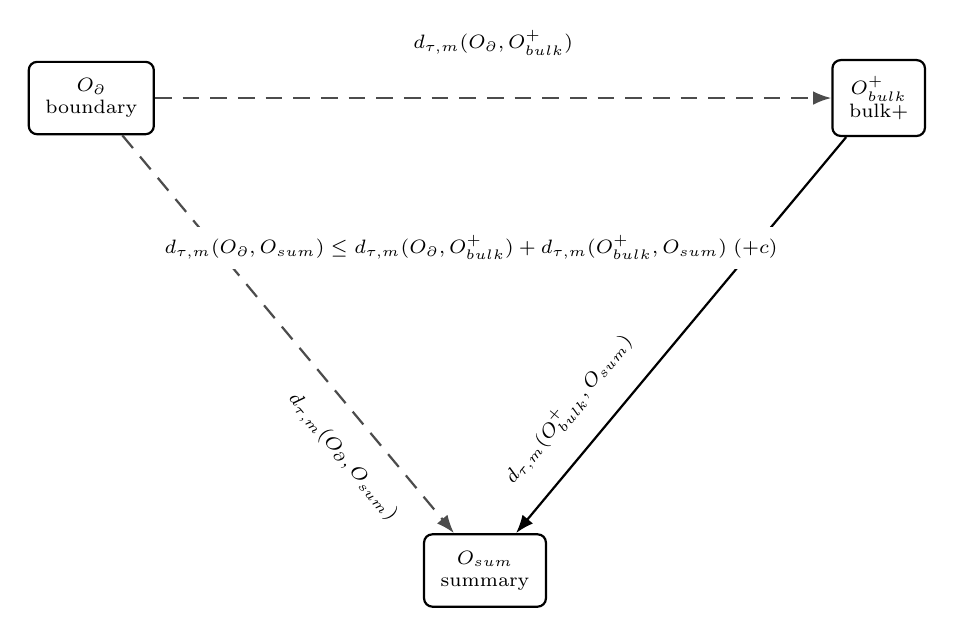
\begin{tikzpicture}[
		      obs/.style={draw=black,thick,rounded corners=3pt,inner sep=6pt,align=center,font=\scriptsize},
		      arr/.style={-Latex,thick,draw=black},
		      maybe/.style={-Latex,thick,draw=black!70,dash pattern=on 6pt off 4pt},
		      >=Latex
		    ]

    \node[obs] (Op) at (0,0) {$O_{\partial}$\\boundary};
    \node[obs] (Ob) at (10.0,0) {$O_{bulk}^{+}$\\bulk$+$};
    \node[obs] (Os) at (5.0,-6.0) {$O_{sum}$\\summary};

    % Draw edges first; add labels afterwards so they are never occluded by the centre inequality box.
    \draw[maybe] (Op) -- (Ob);
    \draw[arr] (Ob) -- (Os);
    \draw[maybe] (Op) -- (Os);

    \node[font=\scriptsize,align=center,text width=10.5cm,fill=white,inner sep=3pt] at (5.0,-1.9)
      {$\begin{aligned}
        d_{\tau,m}(O_{\partial}, O_{sum})
        &\le d_{\tau,m}(O_{\partial}, O_{bulk}^{+})
            + d_{\tau,m}(O_{bulk}^{+}, O_{sum})\;(+c)
      \end{aligned}$};

    % Edge labels (drawn last to sit above the inequality box)
    \path (Op) -- (Ob)
      node[midway,above=5mm,font=\scriptsize,fill=white,inner sep=1pt]
      {$d_{\tau,m}(O_{\partial}, O_{bulk}^{+})$};
    \path (Ob) -- (Os)
      node[pos=0.75,sloped,above=3mm,font=\scriptsize,fill=white,inner sep=1pt]
      {$d_{\tau,m}(O_{bulk}^{+}, O_{sum})$};
    \path (Op) -- (Os)
      node[pos=0.75,sloped,below=3mm,font=\scriptsize,fill=white,inner sep=1pt]
      {$d_{\tau,m}(O_{\partial}, O_{sum})$};

  \end{tikzpicture}
  \caption{Directed translation costs form a Lawvere-style geometry: costs compose additively (triangle inequality),
  asymmetry is expected, and strict budgets can force $+\infty$ distances.
  The dashed arrows emphasise that some translations (e.g.\ boundary$\to$bulk$+$) may be infeasible at fixed $(\tau,m)$.}
  \label{fig:lawvere}
\end{figure}

\subsection{Budget effects: replay is short but not fast}
\label{subsec:rulial-budget-effects}

The boundary/bulk example illustrates why we insist on explicit budgets.

\begin{proposition}[Boundary-to-bulk translation]\label{prop:boundary-bulk}
Let $O_{\partial}$ be a boundary observer and $O_{\mathrm{bulk}}$ a bulk observer as in Example~\ref{ex:boundary-bulk}.
Assume deterministic replay is available as a translator $T_{\mathrm{replay}}$.
Then:
\begin{enumerate}[leftmargin=*]
  \item $\DL(T_{\mathrm{replay}})$ is $O(1)$ relative to the fixed semantics $\Apply$ (it is essentially the interpreter);
  \item for fixed finite budgets $(\tau,m)$, $T_{\mathrm{replay}}\notin\Trans_{\tau,m}(O_{\partial},O_{\mathrm{bulk}})$ once the payload length exceeds $\tau$,
        so $\vec{D}_{\tau,m}(O_{\partial}\!\to\!O_{\mathrm{bulk}})=+\infty$ beyond that regime;
  \item for unbounded budgets, the directed distortion term can be $0$ (exact replay), so
        $\vec{D}_{\infty,\infty}(O_{\partial}\!\to\!O_{\mathrm{bulk}})=O(1)$.
\end{enumerate}
\end{proposition}

\begin{proof}
(1) follows from the fact that the replay algorithm is fixed once the operational semantics is fixed.
(2) is immediate: replay must apply the tick patches sequentially and therefore requires time proportional to payload length.
(3) follows because replay is exact, so distortion vanishes, and only the constant description length remains.
\end{proof}

\begin{remark}[Interpretation]
At unbounded resources, boundary and bulk descriptions may be close in rulial distance.
At bounded resources, they can be infinitely far.
This captures an engineering reality: a short programme can still be computationally infeasible under strict budgets.
In particular, under the two-plane \WARP\ semantics (Paper~II), a state decomposes into a skeleton together with recursively
attached sub-states; translating a boundary observer into a bulk observer amounts to \emph{expanding} these attachment fibres
across the committed tick sequence, work that can be infeasible under strict $(\tau,m)$ budgets.
Wormholes (Paper~III) are precisely provenance-preserving compressions of multi-tick segments into single labelled edges; a bulk observer ``sees inside''
only by replaying (and hence expanding) the corresponding sub-payload.
\end{remark}

\sectionbreak

% ============================================================
\section{Multiway Systems, the Ruliad, and Observer Geometry}
\label{sec:multiway}

We treat the Ruliad connection with full mathematical detail, since later papers in the series
move from mathematics to ethics and architecture.

\subsection[Multiway space induced by warp rewriting]{Multiway space induced by \textnormal{\textsc{Warp}} rewriting}
\label{subsec:multiway-warps}

A rule pack $R$ induces a multiway graph $\MW(\mathcal{U},R)$.
The determinism discipline of Paper~II does \emph{not} remove branching from the underlying multiway space;
rather, it ensures that once a boundary encoding is fixed (initial state, rule pack, scheduler policy, and tie-breaks),
the realised evolution is a unique path.

\begin{figure}[t]
  \centering
  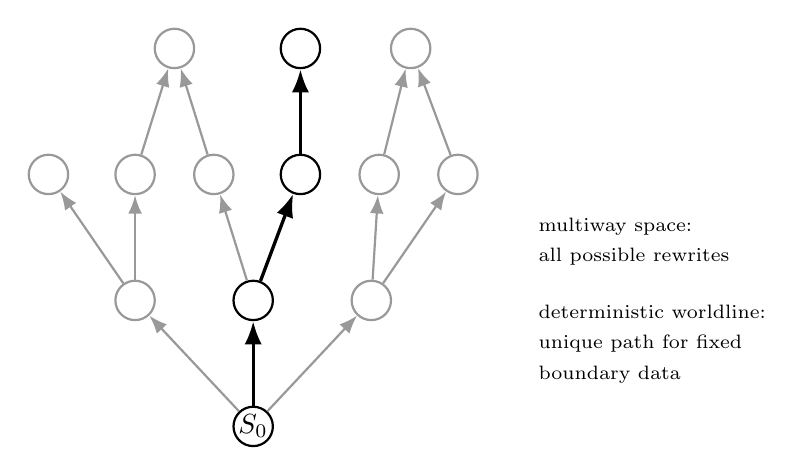
\begin{tikzpicture}[
      state/.style={circle,draw=black,thick,minimum size=5mm,inner sep=0pt},
      ghost/.style={circle,draw=black!40,thick,minimum size=5mm,inner sep=0pt},
      arrow/.style={-Latex,thick,draw=black!40},
      detarrow/.style={-Latex,very thick,draw=black},
      >=Latex
    ]

    % Initial state
    \node[state] (S0) at (0,0) {$S_0$};

    % Level 1
    \node[ghost] (A1) at (-1.5,1.6) {};
    \node[state] (A2) at (0,1.6) {};
    \node[ghost] (A3) at (1.5,1.6) {};

    \draw[arrow]   (S0) -- (A1);
    \draw[detarrow] (S0) -- (A2);
    \draw[arrow]   (S0) -- (A3);

    % Level 2
    \node[ghost] (B1) at (-2.6,3.2) {};
    \node[ghost] (B2) at (-1.5,3.2) {};
    \node[ghost] (B3) at (-0.5,3.2) {};
    \node[state] (B4) at (0.6,3.2) {};
    \node[ghost] (B5) at (1.6,3.2) {};
    \node[ghost] (B6) at (2.6,3.2) {};

    \draw[arrow]   (A1) -- (B1);
    \draw[arrow]   (A1) -- (B2);
    \draw[arrow]   (A2) -- (B3);
    \draw[detarrow] (A2) -- (B4);
    \draw[arrow]   (A3) -- (B5);
    \draw[arrow]   (A3) -- (B6);

    % Level 3 merge points
    \node[ghost] (C1) at (-1.0,4.8) {};
    \node[state] (C2) at (0.6,4.8) {};
    \node[ghost] (C3) at (2.0,4.8) {};

    \draw[arrow]   (B2) -- (C1);
    \draw[arrow]   (B3) -- (C1);
    \draw[detarrow] (B4) -- (C2);
    \draw[arrow]   (B5) -- (C3);
    \draw[arrow]   (B6) -- (C3);

    % Annotation
    \node[anchor=west,align=left] at (3.5,2.35)
      {\scriptsize multiway space:\\[-1pt]
       \scriptsize all possible rewrites};
    \node[anchor=west,align=left] at (3.5,1.05)
      {\scriptsize deterministic worldline:\\[-1pt]
       \scriptsize unique path for fixed\\[-1pt]
       \scriptsize boundary data};

  \end{tikzpicture}
  \caption{A deterministic worldline (thick) through the multiway space of all possible \WARP\ rewrites.
  Fixing the rule pack, initial state, and scheduling/tie-break data selects a unique path; alternative branches
  represent different matches, schedules, or rule-pack choices.}
  \label{fig:multiway-slice}
\end{figure}

\begin{remark}[Confluence vs determinism]
Confluence is a property of a rewrite system: different rewrite orders lead to a common result.
Determinism in Paper~II is stronger and more operational: given fixed boundary data, there is a unique committed tick outcome.
The multiway graph still exists as the ambient possibility space in which observers may reason about counterfactuals.
\end{remark}

\subsection{The Ruliad as a large history space}
\label{subsec:ruliad}

Wolfram's Ruliad is informally the limit of all possible computations; in our setting it is natural to model it
as a large history space built from multiway systems~\cite{Wolfram2020}.

\begin{definition}[Aion/Ruliad history space]\label{def:ruliad}
Fix a class $\mathfrak{R}$ of admissible rule packs and a class $\mathfrak{U}$ of admissible initial states.
Define the \emph{Aion history space} (the \emph{Ruliad} in our setting) as the disjoint union of history categories
\[
  \Ruliad \;:=\; \bigsqcup_{(U_0,R)\in\mathfrak{U}\times\mathfrak{R}} \Hist(\mathcal{U}_{U_0,R},R),
\]
where $\mathcal{U}_{U_0,R}$ is the forward closure of $U_0$ under $R$ (the reachable states).
\end{definition}

\begin{remark}[Large-category caveat]
$\Ruliad$ is a large category (indeed a proper class in many settings).
The disjoint union is deliberate: we treat histories as provenance-bearing artefacts, so components are not quotiented by extensional
state equality.
In particular, even if two reachable states are \emph{identical} as graph-shaped data, we keep them as distinct objects of $\Ruliad$
when they arise from different causal origins (different initial states and/or rule packs).
This contrasts with a ``merging'' view of the Ruliad that identifies states across components and thereby erases origin information.
We use it as a conceptual container: the purpose is to make explicit that a single deterministic worldline is a small, selected path
within a vastly larger possibility space.
None of the metric arguments in \S\ref{sec:rulial} require manipulating $\Ruliad$ as a set-theoretic object.
\end{remark}

\subsection{Chronos, Kairos, Aion}
\label{subsec:chronos-kairos-aion}

We formalise the three-layer time model alluded to in earlier drafts.

\begin{definition}[Chronos]\label{def:chronos}
\emph{Chronos time} is the linear time of a fixed worldline:
given a replayable payload $P=(\mu_0,\ldots,\mu_{n-1})$ of \emph{tick patches}, Chronos is the finite linear order
$0<1<\cdots<n$ on committed ticks, or the functor $\Chronos:[n]\to\Hist(\mathcal{U},R)$ selecting the unique replay path.
If a tick patch $\mu_i$ is internally realised by a within-tick microstep trace, we treat that trace as structure \emph{inside}
the tick edge label rather than as additional Chronos instants.
\end{definition}

\begin{definition}[Kairos]\label{def:kairos}
\emph{Kairos time} is the structure of \emph{branch events}:
points at which alternative continuations exist in the multiway graph (alternative matches, schedules, rule packs, or inputs),
or, internally, points within a tick at which candidate matches conflict (witnessed by the within-tick trace posets of Paper~II).
Formally, Kairos may be modelled as a subgraph (or event structure) of $\MW(\mathcal{U},R)$ capturing divergence and merge loci.
\end{definition}

\begin{definition}[Aion]\label{def:aion}
\emph{Aion time} is the history category $\Hist(\mathcal{U},R)$: the possibility space of all finite derivations in the multiway graph.
At the largest scale, the Ruliad history space $\Ruliad$ (Definition~\ref{def:ruliad}) is the disjoint union of such Aion categories across initial states and rule packs.
\end{definition}

\subsection{Temporal logic on Chronos--Kairos--Aion}
\label{subsec:temporal-logic}

The three-layer time model is most useful when it supports clear \emph{statements} about computation:
safety properties (``nothing bad ever happens''), liveness properties (``something good eventually happens''),
and branch-sensitive claims (``every possible continuation eventually reconciles'').
Temporal logics provide a compact language for such statements~\cite{Pnu77,CES86}.

\paragraph{Atomic propositions are observer-relative.}
In our setting a ``state'' may carry arbitrarily rich provenance and interior structure,
but an observer sees only a trace value.
Accordingly, we interpret atomic propositions as predicates on trace space.
Fix a set $\mathsf{AP}$ of atomic propositions and, for each $p\in\mathsf{AP}$, a predicate (by abuse of notation)
\[
  p \;:\; \Tr \to \{0,1\}.
\]
Given an observer $O:\Hist(\mathcal{U},R)\to\Tr$, we write $O\models_h p$ to mean $p(O(h))=1$
for a history morphism $h\in\Mor(\Hist(\mathcal{U},R))$.

\paragraph{A minimal CTL$^\ast$-style language on histories.}
To engineer reliable systems on top of the Aion possibility space, we require a formal language to state invariants such as
``all branches eventually merge'' or ``provenance is always preserved'', and to reason about how such claims behave under
observer translation.
We evaluate formulas on \emph{history prefixes} rather than bare states, because observers can be path-dependent.
Let $\varphi$ range over \emph{state formulas} and $\psi$ over \emph{path formulas}:
\[
\begin{array}{rcl}
\varphi &::=& p \mid \neg\varphi \mid (\varphi\wedge\varphi) \mid \mathbf{A}\psi \mid \mathbf{E}\psi,\\[2pt]
\psi &::=& \varphi \mid \neg\psi \mid (\psi\wedge\psi) \mid \mathbf{X}\psi \mid \mathbf{F}\psi \mid \mathbf{G}\psi \mid (\psi\ \mathbf{U}\ \psi),
\end{array}
\]
where $p\in\mathsf{AP}$, and $\mathbf{A}$ (``for all paths'') / $\mathbf{E}$ (``there exists a path'') quantify over
continuations in the Aion/multiway space.
The operators $\mathbf{X},\mathbf{F},\mathbf{G},\mathbf{U}$ are read as ``next'', ``eventually'', ``always'',
and ``until'', respectively.

\paragraph{Semantics.}
Write $\MW(\mathcal{U},R)$ for the multiway graph, and interpret a \emph{one-step} extension of a history prefix
$h:U_0\to U$ as composition with a single outgoing rewrite edge $e:U\to U'$ in $\MW$.
A (maximal) \emph{continuation path} from $h$ is then an infinite sequence of such one-step extensions
(or, for finite computations, a finite path padded by stuttering at its terminal object).
We write $h[i]$ for the length-$i$ extension along a continuation, with $h[0]=h$.

State satisfaction $O\models_h\varphi$ and path satisfaction $O\models_{h,\pi}\psi$ (where $\pi$ is a continuation of $h$)
are defined by the standard CTL$^\ast$ clauses:
\begin{itemize}[leftmargin=*]
  \item $O\models_h p$ iff $p(O(h))=1$;
  \item $O\models_h \mathbf{A}\psi$ iff for every continuation $\pi$ of $h$, $O\models_{h,\pi}\psi$;
        and $O\models_h \mathbf{E}\psi$ iff for some continuation $\pi$ of $h$, $O\models_{h,\pi}\psi$;
  \item $O\models_{h,\pi}\mathbf{X}\psi$ iff $O\models_{h[1],\pi}\psi$;
  \item $O\models_{h,\pi}\mathbf{F}\psi$ iff there exists $i\ge 0$ such that $O\models_{h[i],\pi}\psi$;
  \item $O\models_{h,\pi}\mathbf{G}\psi$ iff for all $i\ge 0$, $O\models_{h[i],\pi}\psi$;
  \item $O\models_{h,\pi}(\psi_1\ \mathbf{U}\ \psi_2)$ iff there exists $k\ge 0$ with
        $O\models_{h[k],\pi}\psi_2$ and for all $0\le i<k$, $O\models_{h[i],\pi}\psi_1$.
\end{itemize}
Chronos is recovered by evaluating path formulas along the unique continuation selected by deterministic replay
(Definition~\ref{def:chronos}); Aion semantics uses the full continuation set; and Kairos points are the prefixes $h$
whose endpoint admits multiple distinct one-step extensions (Definition~\ref{def:kairos}).

\begin{example}[Liveness of provenance exposure on Chronos]\label{ex:temporal-liveness}
Let $p_{\mathrm{expose}}\in\mathsf{AP}$ be the atomic proposition ``a specified provenance receipt has been exposed'',
defined as a predicate on trace space (e.g.\ the trace contains a receipt hash, or a certificate has been emitted).
On a fixed deterministic worldline, the liveness claim
\[
  \mathbf{G}\,\mathbf{F}\,p_{\mathrm{expose}}
\]
asserts that \emph{at every time}, exposure eventually occurs again.
This is an instance of an ``always eventually'' property: exposure may be delayed by compression or batching,
but it cannot be postponed indefinitely along Chronos.
\end{example}

\begin{example}[Eventual reconciliation across branches]\label{ex:temporal-reconcile}
Let $p_{\mathrm{merge}}$ be the proposition ``the current prefix lies at (or after) a merge locus'',
for example detected by the multiway graph structure or by a trace witness of branch reconciliation.
The Aion-level claim
\[
  \mathbf{A}\,\mathbf{F}\,p_{\mathrm{merge}}
\]
says that \emph{every} possible continuation from the current prefix eventually reaches a merged regime.
In contrast, $\mathbf{E}\,\mathbf{F}\,p_{\mathrm{merge}}$ asserts only that \emph{some} continuation eventually reconciles,
which is strictly weaker when divergence is possible.
\end{example}

To ensure temporal claims are stable under small representation-level discrepancies between traces, we will assume a $\delta$-robustness condition on atomic propositions.

\begin{proposition}[Temporal properties transport along low-distortion translation]\label{prop:temporal-transport}
Fix $\delta\ge 0$ and assume each atomic proposition $p\in\mathsf{AP}$ is \emph{$\delta$-robust} in trace space:
whenever $\mathrm{dist}_{\mathrm{tr}}(t,t')\le\delta$ we have $p(t)=p(t')$.
Let $O_1,O_2$ be observers and let $T\in\Trans_{\tau,m}(O_1,O_2)$ satisfy
\[
  \Dist(O_2,\,T\circ O_1)\le \delta.
\]
Then for every history prefix $h$ and every state formula $\varphi$ in the above language,
\[
  O_2 \models_h \varphi
  \quad\Longleftrightarrow\quad
  (T\circ O_1)\models_h \varphi.
\]
Likewise, for every continuation $\pi$ of $h$ and every path formula $\psi$,
\[
  O_2 \models_{h,\pi} \psi
  \quad\Longleftrightarrow\quad
  (T\circ O_1)\models_{h,\pi} \psi.
\]
In particular, temporal truth in $O_2$ can be decided from $O_1$ by applying an admissible translator whose cost is controlled by
the directed hom-value $d_{\tau,m}(O_1,O_2)$ (Definition~\ref{def:lawvere-hom}) and hence by $D_{\tau,m}$ (Definition~\ref{def:rulial}).
\end{proposition}

\begin{remark}[Robustness in practice]
The $\delta$-robustness hypothesis is mathematically clean, but it can be strict for discrete trace structures
(hashes, exact logs, serialisations): a tiny change in representation can flip an atomic predicate.
In practice, robustness is enforced by canonicalisation or coarse-graining of traces before predicate evaluation.
We then define propositions on such a canonicalised or coarse-grained view of the trace
(normalising order, discarding nonce-like fields, bucketing timestamps), or we use approximate matching,
so that minor log variation does not alter the high-level truth values being checked.
Conversely, if an observer suppresses events relevant to a predicate (for example by strong summarisation), then either the predicate is not $\delta$-robust under the chosen trace metric or the translation distortion exceeds $\delta$; Proposition~\ref{prop:temporal-transport} is intentionally restricted to the robust regime.
\end{remark}

\begin{proof}
The hypothesis $\Dist(O_2,T\circ O_1)\le\delta$ means that for every history prefix $h$,
\[
  \mathrm{dist}_{\mathrm{tr}}\bigl(O_2(h),\,T(O_1(h))\bigr)\le\delta.
\]
By $\delta$-robustness, all atomic propositions have identical truth values under $O_2$ and $T\circ O_1$ at every prefix.
Since the temporal semantics above depends only on these pointwise truth values along continuations,
the equivalence follows by induction on the structure of formulas.
More explicitly, the equivalence follows by structural induction on formulas: boolean connectives preserve equivalence immediately, and the temporal operators ($\mathbf{X},\mathbf{F},\mathbf{G},\mathbf{U}$)
and path quantifiers ($\mathbf{A},\mathbf{E}$) depend only on truth values at successive prefixes, which by hypothesis agree pointwise between
$O_2$ and $T\circ O_1$.
\end{proof}

\subsection{Observer geometry as frame separation in the Ruliad}
\label{subsec:ruliad-geometry}

Within $\Ruliad$, an observer is a functor that assigns traces to histories.
Two observers may differ substantially on causal structure, yet still be near each other in rulial distance when translation cost is low under the given budgets.
Conversely, two observers may agree semantically but be distant if the only translation requires large algorithmic overhead under the given budgets.

The temporal-logic layer of \S\ref{subsec:temporal-logic} makes this observer-dependence explicit:
atomic propositions live on trace space, so temporal truth is phrased in what a given observer can \emph{see}.
Proposition~\ref{prop:temporal-transport} then formalises when such temporal claims transport across observers:
low-distortion translation preserves satisfaction for robust predicates.
Meanwhile, the Lawvere-enriched viewpoint of \S\ref{subsec:lawvere} reinterprets directed translation costs as enriched hom-values,
so that ``translation geometry'' is precisely the compositional structure encoded by the triangle inequality.

A central point is technical: \emph{rulial distance is not a semantic truth predicate}; it is a geometry induced by translation constraints.
In this sense, it is analogous to choosing a coordinate chart in physics: an ill-conditioned chart can make simple structure appear complex.

\begin{remark}[Rulial balls and neighbourhoods]
Given an observer $O$ and radius $r$, the \emph{rulial ball} $B_r(O)=\{O':D_{\tau,m}(O,O')\le r\}$
collects observers mutually reachable within a fixed translation cost.
This provides a mathematically explicit way to talk about ``nearby frames'' without privileging a single canonical observer.
\end{remark}

\subsection{Engineering implication}
The observer geometry is not merely a matter of exposition.
It provides a quantitative tool for system design:
if a compliance observer is far from a diagnostic observer under deployment budgets,
then emitting only compliance traces is not a neutral optimisation --- it is a choice that can make subsequent diagnosis prohibitively expensive or impossible.
Conversely, if a summary observer is close to a full-bulk observer under expected budgets, we may deploy summary traces
without forfeiting the ability to reconstruct details when required.
Equivalently, we choose a deployed observer $O$ so that the required secondary views lie within a small rulial ball $B_r(O)$ under the relevant budgets.

\paragraph{Computability.}
In full generality, $D_{\tau,m}$ is defined by an infimum over all admissible translator programmes; like other Kolmogorov/MDL-flavoured optima,
it is a useful \emph{specification} but not something we claim to compute exactly in a deployed system.
The engineering task is to construct explicit translators.
We then use these concrete translators to bound the mathematical distance from above, rather than attempting to evaluate the infimum itself.
Concretely, we build a specific translator $T_{12}$ (and, if needed, $T_{21}$), measure or estimate its resource usage under $(\tau,m)$, and use
\[
  \DL(T_{12}) + \lambda\,\Dist(O_2,\,T_{12}\circ O_1)
\]
as a computable upper bound on the directed cost $\vec{D}_{\tau,m}(O_1\!\to\! O_2)$ (and similarly in the reverse direction, yielding an upper bound on $D_{\tau,m}$).
This turns rulial distance from an abstract infimum into an actionable design parameter: constructing better translators tightens these bounds.

\sectionbreak

% ============================================================
\section{Related Work}
\label{sec:related}

\paragraph{Multiway systems and the Ruliad.}
Wolfram introduces multiway systems and the Ruliad as a framework for fundamental physics and metamathematics~\cite{Wolfram2020}.
Our \WARP\ rewriting induces multiway graphs directly; our determinism discipline selects unique worldlines within this possibility space.
The rulial distance is our contribution to the specific problem of quantifying observer differences.

\paragraph{Minimum Description Length.}
The MDL principle, pioneered by Rissanen~\cite{Ris78}, provides an information-theoretic basis for balancing model complexity and fit.
We apply MDL to measure translator complexity. Connections to prefix complexity and invariance are treated classically in the literature on
Kolmogorov complexity~\cite{LiVitanyi2019}; we require only the constant-overhead subadditivity property.

\paragraph{Categorical computation and diagrammatic reasoning.}
String diagrams and categorical algebra have been applied successfully to concurrency and quantum computing~\cite{CD11}.
Our two-plane view of \WARP\ state (skeleton plus attachment fibres) sits in this tradition: attachments live in fibres, and reindexing along skeleton morphisms
transports attachment updates coherently. The novelty is not any single component, but the synthesis across recursion, rewriting, determinism, and provenance.

\sectionbreak

% ============================================================
\section{Discussion and Outlook}
\label{sec:outlook}

This paper completes the mathematics-oriented foundations of \AION{} by making observer-dependence explicit and computable.
Taken together, Papers~I--IV trace a single line: \emph{structure} (recursive \WARP\ state), \emph{dynamics} (deterministic worldlines),
\emph{provenance} (holographic boundary payloads), and finally \emph{geometry} (rulial distance on observers).
Deterministic replay and holographic provenance mean the same computation can be represented compactly in many forms.
Rulial distance turns the question ``how different are these forms?'' into a quantitative, resource-aware statement.

Several directions remain open, but they are now delineated:
\begin{itemize}[leftmargin=*]
  \item \textbf{Ethics (Paper V).} Once perfect provenance and deterministic replay are available, the principal questions shift from mathematics to governance.
        When provenance records cognitive processes---whether of autonomous digital agents or hybrid human--AI systems---replay becomes an ethically significant act,
        not a neutral debugging primitive.
        Paper~V develops \emph{provenance sovereignty}: an agent's right to control capture, inspection, replay, and branching of its worldline.
        We extract runtime-level requirements (consent, revocation, capability-scoped observers, cryptographic sealing, and fork rights) and show how they constrain
        the design of replay tooling and provenance payload formats.
  \item \textbf{Architecture (Paper VI).} The system design question is how to build a machine whose primitive step is a provenance-carrying \WARP\ rewrite,
        with efficient storage, slicing, and multiverse debugging.
\end{itemize}

On the mathematical side, this paper adds two complementary lenses:
a minimal temporal logic aligned with Chronos--Kairos--Aion (\S\ref{subsec:temporal-logic}),
and a Lawvere-metric/enriched-category view of directed translation costs (\S\ref{subsec:lawvere}).
Further work may refine these foundations in three directions:
(i) develop fully directed rulial quasi-metrics without symmetrisation and with tighter control of $O(1)$ slack;
(ii) study quantitative/robust temporal predicates and efficient model checking on \WARP\ history spaces; and
(iii) work out the enriched-categorical completion theory (Yoneda, Cauchy completion) and its computational meaning for observer limits.

\sectionbreak

% ============================================================
\section{Notation Summary}
\label{sec:notation}

\begin{center}
\begin{tabularx}{\linewidth}{lX}
  Symbol & Meaning \\ \hline
  $\mathcal{U}$ & a \WARP\ universe (collection of states) \\
  $\WState$ & class/category of \WARP\ states \\
  $\Labels$ & space of tick patches \\
  $\Apply$ & deterministic tick-application function $\WState \times \Labels \rightharpoonup \WState$ \\
  $R$ & rule pack / rewrite rule set \\
  $\MW(\mathcal{U},R)$ & multiway graph induced by rewriting \\
  $\Hist(\mathcal{U},R)$ & history category (path category of $\MW$) \\
  $(\Tr,\mathrm{dist}_{\mathrm{tr}})$ & trace space with trace distortion metric \\
  $O:\Hist(\mathcal{U},R)\to\Tr$ & observer (functor to traces) \\
  $T:\Tr\to\Tr$ & translator acting by post-composition \\
  $\Trans_{\tau,m}(O_1,O_2)$ & translators from $O_1$ to $O_2$ within budgets $(\tau,m)$ \\
  $\DL(T)$ & MDL description length of translator $T$ \\
  $c$ & subadditivity constant (Assumption~\ref{ass:dl-subadd}) \\
  $\lambda$ & weighting parameter trading off $\DL$ vs.\ distortion \\
  $\Dist(O,O')$ & lifted observer distortion (supremum over histories) \\
  $\vec{D}_{\tau,m}(O_1\!\to\!O_2)$ & directed rulial cost \\
  $d_{\tau,m}(O_1,O_2)$ & the same quantity, viewed as a Lawvere hom-value \\
  $D_{\tau,m}(O_1,O_2)$ & symmetrised rulial distance \\
  $B_r(O)$ & rulial ball of radius $r$ around observer $O$ \\
  $\mathrm{BTR}$ & Boundary Transition Record (Paper~III) \\
  $O\models_h \varphi$ & temporal satisfaction at history prefix $h$ \\
  $\mathbf{A},\mathbf{E},\mathbf{X},\mathbf{G},\mathbf{F},\mathbf{U}$ & temporal operators (all/exists paths; next/always/eventually/until) \\
  $\Chronos$ & linear time of a fixed worldline; functor $[n]\to\Hist(\mathcal{U},R)$ \\
  $\Kairos$ & branch-event structure; subgraph of $\MW$ capturing divergence loci \\
  $\Aion$ & encompassing possibility space; full history category or Ruliad \\
  $\Ruliad$ & Ruliad/Aion history space (large union of histories) \\
\end{tabularx}
\end{center}

\sectionbreak

\appendix
\section*{Appendix A. A worked example of rulial distance}

This appendix provides a small concrete example illustrating how rulial distance is used in
practice. The purpose is not to compute an exact infimum in Definition~\ref{def:rulial}, but to demonstrate
how explicit translators yield computable upper bounds on observer separation.

\subsection*{A.1 Setup}

Consider a deterministic \WARP\ worldline consisting of three committed ticks:
\[
U_0 \xRightarrow{\mu_0} U_1 \xRightarrow{\mu_1} U_2 \xRightarrow{\mu_2} U_3 .
\]
Let the boundary encoding be $(U_0, P)$, where the provenance payload is
\[
P = (\mu_0, \mu_1, \mu_2).
\]

We consider two observers of histories in $\Hist(\mathcal{U},R)$:
\begin{itemize}
\item the \emph{boundary observer} $O_\partial$, which maps any history prefix to the compact
boundary artefact $(U_0,P)$; and
\item the \emph{bulk observer} $O_{\mathrm{bulk}}$, which maps a history prefix to the explicit
state sequence, bundled with the boundary artefact, $(U_0,P,U_1,U_2,U_3)$.
\end{itemize}

\paragraph{Trace space clarification.}
In this example, the trace space $\Tr$ is taken large enough to include both boundary artefacts $(U_0,P)$ and
explicit state sequences.
We equip $\Tr$ with a metric that yields zero distortion when traces agree up to representation or formatting.
This makes the zero-distortion claims below immediate.

Both observers are deterministic and well-defined on all prefixes of the committed worldline.

\subsection*{A.2 Translators}

There are two natural translators between these observers.

\begin{enumerate}
\item \textbf{Forgetful projection.}
\[
T_{\mathrm{forget}} : O_{\mathrm{bulk}} \to O_\partial,
\]
which extracts the boundary artefact $(U_0,P)$ from the bulk trace. This translator has constant
description length,
\[
\DL(T_{\mathrm{forget}}) = O(1),
\]
and zero residual distortion, since the boundary payload is already present in the bulk
representation.

\item \textbf{Replay expansion.}
\[
T_{\mathrm{replay}} : O_\partial \to O_{\mathrm{bulk}},
\]
which deterministically replays the payload $P$ using the fixed semantics
$\Apply$. Its description length is also constant relative to the fixed interpreter,
\[
\DL(T_{\mathrm{replay}}) = O(1),
\]
but its runtime cost grows linearly with $|P|$.
\end{enumerate}

\subsection*{A.3 Directed rulial costs}

Fix budgets $(\tau,m)$.

\begin{itemize}
\item For sufficiently small $\tau$, replay is infeasible:
$T_{\mathrm{replay}} \notin \Trans_{\tau,m}(O_\partial,O_{\mathrm{bulk}})$.
Hence
\[
\vec{D}_{\tau,m}(O_\partial \to O_{\mathrm{bulk}}) = +\infty .
\]

\item In the reverse direction, $T_{\mathrm{forget}}$ is admissible under any budget, with zero
residual distortion, yielding (for any $\lambda>0$)
\[
\vec{D}_{\tau,m}(O_{\mathrm{bulk}} \to O_\partial) = O(1).
\]
\end{itemize}

For unbounded budgets $(\tau,m)=(\infty,\infty)$, replay is admissible and exact, so both directed
costs are $O(1)$.
Here the hidden constant is independent of $|P|$ (history length) once the fixed semantics $\Apply$ and the translator coding scheme are chosen.

\subsection*{A.4 Symmetrised distance}

The symmetrised rulial distance is
\[
D_{\tau,m}(O_\partial,O_{\mathrm{bulk}})
= \vec{D}_{\tau,m}(O_\partial \to O_{\mathrm{bulk}})
+ \vec{D}_{\tau,m}(O_{\mathrm{bulk}} \to O_\partial).
\]

Thus:
\begin{itemize}
\item under strict budgets,
$D_{\tau,m}(O_\partial,O_{\mathrm{bulk}})=+\infty$; and
\item under relaxed budgets,
$D_{\infty,\infty}(O_\partial,O_{\mathrm{bulk}})=O(1)$.
\end{itemize}

\subsection*{A.5 Interpretation}

This example illustrates the operational use of rulial distance. In practice we do not compute the
infimum in Definition~\ref{def:rulial} directly; rather, we construct explicit translators and thereby obtain
concrete upper bounds. Improving translators reduces these bounds, whereas strong summarisation
or information hiding can increase them---in the limiting case, to $+\infty$. The geometry therefore captures
how observer separation depends on available resources rather than on semantic disagreement.

\clearpage
\addcontentsline{toc}{section}{References}
\bibliographystyle{alphaurl}
\bibliography{refs}

\end{document}
